\documentclass[fleqn,10pt]{wlscirep}
\usepackage[utf8]{inputenc}
\usepackage[T1]{fontenc}
\usepackage{algorithm,algpseudocode}
\usepackage{mathtools}
\usepackage{epstopdf}
\epstopdfDeclareGraphicsRule{.tif}{png}{.png}{%
	convert #1 \OutputFile         
}
\DeclarePairedDelimiter\ceil{\lceil}{\rceil} 
\title{Pattern matching based denoising for images with repeated sub strucutures.}

\author[1,*]{Alice Author}
\author[2]{Bob Author}
\author[1,2,+]{Christine Author}
\author[2,+]{Derek Author}
\affil[1]{Affiliation, department, city, postcode, country}
\affil[2]{Affiliation, department, city, postcode, country}

\affil[*]{corresponding.author@email.example}

\affil[+]{these authors contributed equally to this work}

%\keywords{Keyword1, Keyword2, Keyword3}

\begin{abstract}
Example Abstract. Abstract must not include subheadings or citations. Example Abstract. Abstract must not include subheadings or citations. Example Abstract. Abstract must not include subheadings or citations. Example Abstract. Abstract must not include subheadings or citations. Example Abstract. Abstract must not include subheadings or citations. Example Abstract. Abstract must not include subheadings or citations. Example Abstract. Abstract must not include subheadings or citations. Example Abstract. Abstract must not include subheadings or citations.
\end{abstract}
\begin{document}

\flushbottom
\maketitle
% * <john.hammersley@gmail.com> 2015-02-09T12:07:31.197Z:
%
%  Click the title above to edit the author information and abstract
%
\thispagestyle{empty}

\noindent Please note: Abbreviations should be introduced at the first mention in the main text – no abbreviations lists. Suggested structure of main text (not enforced) is provided below.

\section*{Introduction}

Transmission Electron Microscopy (TEM) imaging has been helpful to solve numerous scientific questions in life and material sciences \cite{CURRY200691}$^{,}$\cite{WANG2008395} . However, at times the noise in the acquired images corrupt the signal beyond a useful level. Noise in images can appear due to intrinsic reasons like problems in the sensors or the digital circuits, or due to external factors like the environment. Image denoising plays a vital role especially in suppressing microscopy image noise.

The TEM imaging contrast is based on the interaction between specimen and a multi keV electron beam. While the optical resolution for modern TEM system can be below one angstrom, the high energy electrons often lead to a fast degradation of the sample. For such samples only few electrons can be used for imaging. This leads to a degradation of the images resolution, thus making the image hard to interpret. Therefore after image acquisition, numerical processing is required to enhance the image quality.

To get maximal image quality with minimal dose, various image denoising algorithms were proposed in the past. Conventional denoising methods\cite{bcm_nlm}$^{,}$ \cite{DBLP:journals/tip/BM3D} use only noisy images for the denoising task, whereas most modern methods involving a deep neural network\cite{zhang2018ffdnet}$^{,}$ \cite{zhang2017beyond} require clean images as ground truths for training. Since clean electron microscopy images are not available in most cases, modern denoising methods that require clean images as ground truths cannot be used. However, there are also some deep neural network based methods that use noisy supervision\cite{DBLP:journals/corr/abs-1803-04189} and self supervision\cite{krull2019noise2void} . Although, conventional and self-supervised methods have shown success in denoising images, these methods improved the denoising quality only by a relatively small margin for images with repeated patterns. Hence, a new denoising algorithm is proposed and its results are analyzed and compared with the state-of-the-art methods showing significant gain in image quality. 


\section*{Method}

The proposed denoising algorithm identifies similar patches within the entire image and averages them to suppress the noise. Averaging patches with similar information suppresses noise that is randomly distributed. Since the noise is assumed to be having zero mean, it cancels out when multiple patches are averaged. However the base signal remains the same throughout and averaging does not disrupt the signal. Hence combining different patches result in the denoised image, close to the actual signal value. 

Let $x_{i}$ be the $i^{th}$ noisy patch, $k$ be the number of patches that are averaged, $s_i$, and $n_i$ be the signal and noise in the $i^{th}$ patch respectively. Then,
\begin{equation}
	x_i = s_i + n_i
\end{equation}
Averaging over $k$ patches results in an expected value,
\begin{equation}
	E[\frac{1}{k}\sum_{i}^{k}x_i ] = E[\frac{1}{k}\sum_{i}^{k}(s_i + n_i) ]
\end{equation}
Since the noise is expected to be having zero mean and the base signal is expected to be the same, this ideally means that,
\begin{equation}
	E[\frac{1}{k}\sum_{i}^{k}x_i ] = s
\end{equation}
Hence the variance of the averaged patch is small, i.e,
\begin{equation}
	Var[\frac{1}{k}\sum_{i}^{k}x_i ] = \frac{1}{k^2 -1} \sum_{i}^{k}Var(n_i)
\end{equation}
since $Var(s_i) = 0$ for all $i$. Hence averaging patches with the same signal suppresses noise.

%The basic idea of the algorithm can be compared with the Single Particle Imaging \cite{bhushan_single_2017}, which is an image processing technique used to analyze low dose Transmission Electron Microscopy (TEM) images of identical but dose sensitive samples. Images of specimens obtained from TEM are often very noisy, and hence it is difficult to interpret the information contained in the image. Averaging several images of the same specimen can remove random noise and make the information more interpretable \cite{bhushan_single_2017}.

%It can also be said that this algorithm is similar to the Non-Local Means \cite{bcm_nlm} algorithm in some aspects. In Non-Local Means, similar patches are found only from the immediate surroundings, where as the region of interest is not restricted in the proposed denoising algorithm. Increasing the search space in Non-Local Means has a massive impact on the computation speed. 

\subsection*{Outline of the proposed algorithm}

\begin{figure}
	\centering
	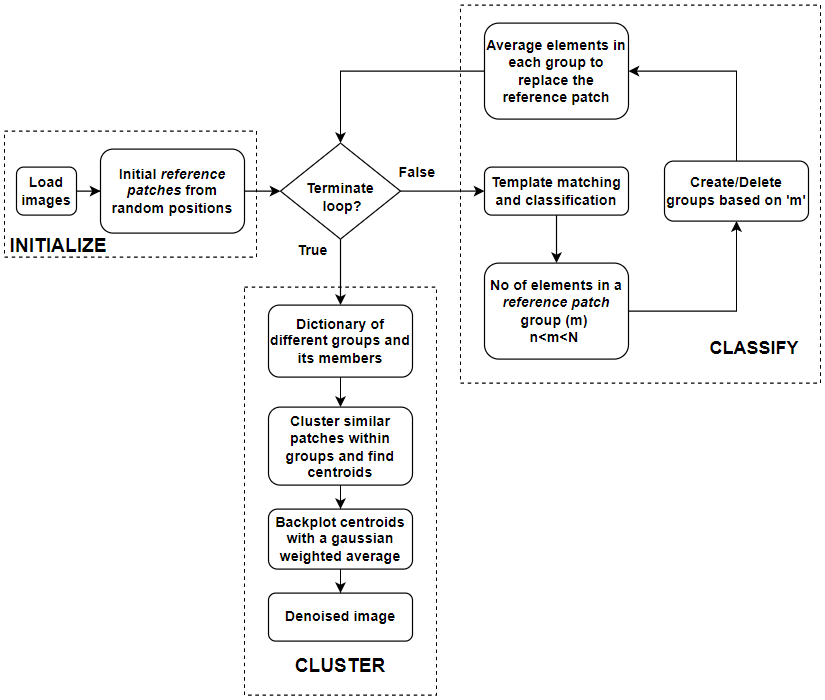
\includegraphics[scale=0.7]{./imgs/flowchart.png}
	\caption{Flowchart of the algorithm}
	\label{fig:flowchart}
\end{figure} 

The proposed algorithm groups similar patches at two levels. Normalized convolution is used to broadly group similar patches within an image and clustering is used to more finely group closely matching patches within the groups obatined during the first step. The flowchart of the algorithm is shown in figure \ref{fig:flowchart} and the two levels of pattern matching is represented by `classify' and `cluster' sections of the flowchart.

Normalized convolution between a template and an image results in local cosine similarity. Cosine similarity  measures similarities between two vectors\cite{alake_understanding_2021} by finding the cosine of the angle between them. If the vectors are in the same direction (i.e., similar), cosine similarity is maximal. It is mathematically represented as,
\begin{equation}
	similarity = cos(\theta) = \frac{A\cdot B}{\|A\|\|B\|} = \frac{\sum_{i=1}^{n}A_i B_i}{\sqrt{\sum_{i=1}^{n}A_i^2}\sqrt{\sum_{i=1}^{n}B_i^2}}
\end{equation}
where $A$ and $B$ are two vectors, and $\theta$ is the angle between them. The cosine similarity value lies between -1 and 1. This is similar to the result obtained by template matching , which is represented in figure \ref{fig:template_matching}. An image, a template taken from the image, and the corresponding result can be seen in figure \ref{fig:template_matching}. The maximum value in the result which is marked in red, represents the template’s location in the image. It corresponds to the top-left corner of the template. Values close to the maximum represent the patches similar to the template. Hence cosine similarity can be used to match patches with images, similar to template matching.

%For the proposed algorithm, normalized convolution between a template and an image results in local cosine similarity. This is similar to the result obtained by template matching. Figure \ref{fig:template_matching} demonstrates the working of the template-matching algorithm. An image, a template taken from the image (i.e., \textit{reference patch} in this algorithm), and the corresponding result have been shown. The maximum value in the result which is marked in red, represents the template’s location in the image. It corresponds to the top-left corner of the template. Values close to the maximum represent the patches similar to the template. Hence cosine similarity can be used to match patches with images, similar to template matching. 



\begin{figure}
	\centering
	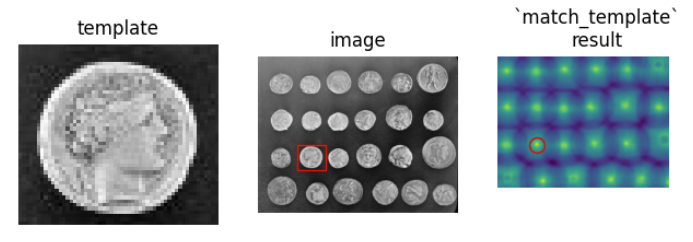
\includegraphics[scale=0.8]{./imgs/template_matching.png}
	\caption[Template matching example]{Template matching example \footnote{\footnotemark} }
	\label{fig:template_matching}
\end{figure} 

\footnotetext{\url{https://scikit-image.org/docs/dev/auto_examples/features_detection/plot_template.html}}

The time complexity of the convolution operation is $O(m^2n^2)$, where $m*m$ is the size of the patch and $n*n$ is the size of the image, which is for large $m$ worse than the run-time of the template matching algorithm. Complexity of the template matching algorithm is $O(n^2log(n^2))$ \cite{template_matching}, where $n*n$ is the image size. Since the convolution operation is widely used in convolutional neural networks, there are Python libraries that support GPU computation for performing the convolution operation. Running the computations on the GPU makes the algorithm much faster.

The algorithm begins with the initialization of random patches of size $m*m$, which are used for matching other patches of size $m*m$ in the image. The patches that are used as templates for matching are referred to as \textit{reference patches}. One example for the initial choice of \textit{reference patches} can be seen in figure \ref{fig:initial_reference_patches}. 

\begin{figure}
	\centering
	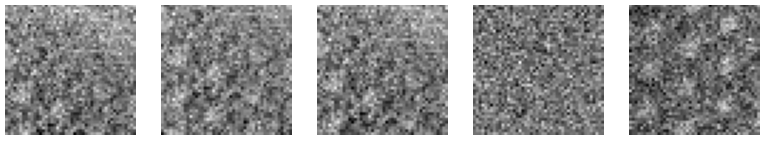
\includegraphics[scale=0.75]{./imgs/initial_reference_patches.png}
	\caption[Initial \textit{reference patches}]{Initial \textit{reference patches} (of size 46*46 pixels), taken from different regions of the input image}
	\label{fig:initial_reference_patches}
\end{figure} 

In the `classify'  section shown in figure \ref{fig:flowchart}, the patches at every position in the image are classified into different groups based on the \textit{reference patch} using cosine similarity. When the cosine similarity is applied, each of patches of size $m*m$ in the image is compared with every other $m*m$ \textit{reference patch}. The result has values between -1 and 1 as the results are normalized. The location with a perfect match is represented by value 1. The patches similar to the \textit{reference patch} are represented by values close to 1. 

Cosine similarity is carried out with all $n$ \textit{reference patches} and all the results are stacked into an array. From this array, the best fitting reference patch index at every position can be determined. Now, the patches in the image that are most similar to the \textit{reference patches} are identified and grouped together.   

%When cosine similarity is carried out with $n$ \textit{reference patches}, result of shape $(p-m+1)*(q-m+1)$ are obtained for each \textit{reference patch}. These results are stacked into an $n*(p-m+1)*(q-m+1)$ array. From this array, the \textit{reference patch} that matches the best at every location is identified. Hence, the $n*(p - m + 1) * (q - m + 1)$ array is reduced to a $(p-m+1)*(q-m+1)$ array which contains the best fitting\textit{ reference patch} index at every position. Now, patches in the image similar to the \textit{reference patches} are identified. The patches represented by the same \textit{reference patch} form a group.

%Although patches at every location are classified to belong into a group, all these patches are not considered. The patches which have a strong correlation with one of the \textit{reference patches} are prioritized. This is done by selecting patches that are close to the maxima in the template matching result. When these patches with strong correlation are selected, the patches around them in the close neighborhood are deleted. That is, if a patch is selected from $(x, y)$, then no patches in the region from $(x-a$ to $x+a, y-a$ to $y+a)$ are selected, where $(a \approx m/4)$ with $m*m$ being the patch size. This gap between patches is used to remove redundant information. Removing redundant information improves the computation speed without affecting the denoising quality.

In the next step, the newly formed groups are deleted or split into more groups based on the group size. The reasoning behind this process is that groups with few members contribute hardly to any denoising, while overly large groups might lead to a loss of detail.  Finally, for each group the old \textit{reference patch} is replaced by the average of all the members in that group. In the next iteration, cosine similarity and the classification steps repeat with these new \textit{reference patches}. We choose to terminate the “classify” section when the total number of reference patches in three consecutive iterations remains the same. Figure \ref{fig:final_reference_patches} shows the reference patches generated after 15 iterations. On comparing figure 1 and figure 4, one can observe that the noise in the final reference patches has been significantly suppressed.

%Once groups of similar patches are formed, the groups are deleted or split into more groups based on the member size. This is because that if the group size is small, there is hardly any denoising effect. On the other hand, if the group size is too big, there can be artifacts generated during averaging due to increased variance. Each of the old \textit{reference patches} is now replaced by the average of all the members in that group. In the next iteration, cosine similarity and the classification steps repeat with these new \textit{reference patches}. One can observe that every iteration may generate new \textit{reference patches}. New \textit{reference patches} are generated when big groups are split into smaller groups. The ``classify” section terminates when the total number of \textit{reference patches} in three consecutive iterations remains the same. Figure \ref{fig:final_reference_patches} shows the \textit{reference patches} generated after 15 iterations. On comparing figure \ref{fig:initial_reference_patches} and figure \ref{fig:final_reference_patches}, one can observe that the noise in the final \textit{reference patches} has been suppressed.

\begin{figure}
	\centering
	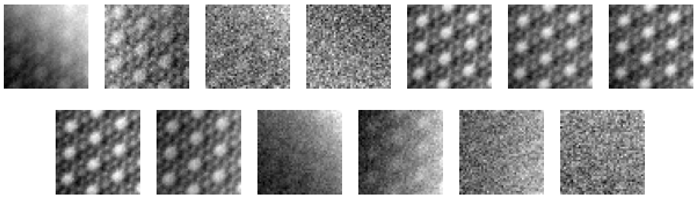
\includegraphics[scale=0.8]{./imgs/final_reference_patches.png}
	\caption{Final \textit{reference patches}}
	\label{fig:final_reference_patches}
\end{figure} 

If the final \textit{reference patches} are used for back plotting (i.e. to replace the patches in their corresponding groups), there are still some artifacts (as shoown ) present because of the following reasons. 

%After running the ``classify” section multiple times, the final \textit{reference patches} are used to replace the patches in their corresponding groups. The denoised image is constructed by using these final \textit{reference patches}. Since \textit{reference patches} can overlap during reconstruction, a $2D$ Gaussian weight is used. The information at the center of a patch is important than the edges. While back plotting, if multiple patches overlap, a weighted average is done. Weighted average with Gaussian weights ensures that the back plotted images do not have sharp edges from the patches used, as the information from the patch edges is suppressed. The back plotted image can be seen in figure \ref{fig:backplot-1}. The following can be inferred from the back plot:

\begin{itemize}
	\item There can be patches in a group that are less similar to the \textit{reference patch}. When these dissimilar patches are averaged, the average might differ from the actual patch by a large extent. 
	\item Cosine similarity is only sensitive to the structure for any two patches which only differ by a constant positive. Therefore, back ploting might not recover local brightness variations.
\end{itemize}

These problems can be solved by averaging over a small group with very closely matched patches. To achieve this, clustering is applied within every group (represented by the final \textit{reference patch}) to create smaller subgroups. The number of clusters in a group can be adjusted by a user set parameter. In other words, the signal-to-noise ratio can be adjusted by changing this parameter value. While previously the whole group was represented by a single \textit{reference patch}, it is now represented by the centriods of the subgroups due to the clustering. Centroids are back plotted with a $2D$ Gaussian weighted average. Gaussian weight smoothens the edges of the centroids, thus preventing artifacts in the reconstructed image. 

A pseudo implementation of the algorithm is shown in the additional information section \ref{algorithm:denoising_algorithm}. The implementation of the denoising algorithm can be found on github\footnote{\url{https://github.com/mbanil/img-denoiser}}.

\subsection*{Parameters of the algorithm and stability}

The algorithm requires a few parameters which the users can tune in order to get optimal performance. Size of the features defined by patch size, position of the initial patches and depending on the amount of denoising desired, the upper and lower limit of the group size for cosine similarity classification can be defined. Finally, the group size for clustering can also be adjusted. This is closely related to the desired signal to noise enhancement. If the user desires an improvement of approximately $N$, the average number of elements in a subgroup should be $N^2$.


%The following are the algorithm parameters.

%\begin{itemize}
%	\item \textbf{Size of the patches}: Patches represent features in an image. Patch sizes should neither be too small nor too large. A patch size of $46*46$ performed the template matching task reasonably well, and hence this was the size used for most of the experiments. 
	
%	\item \textbf{Position of the initial patches}: The position of the initial \textit{reference patches} has to be selected such that the patches represent different regions in the image. These dissimilar patches are selected by randomly initializing the templates such that no two templates are close to each other.
	
%	\item \textbf{Minimum number of patches in a group}:  When there are very few patches, averaging them will not significantly suppress the noise. Hence groups with members lesser than this value are deleted.
	
%	\item \textbf{Maximum number of patches in a group}: The maximum number of patches in a group (represented by a \textit{reference patch}) is set to 100. The first reason is to avoid over-generalization. If the group size is big, a single \textit{reference patch} will represent too many patches, which is undesirable. 
	
%	More groups are generated if this parameter has a lower value, resulting in more \textit{reference patches}. The number of \textit{reference patches} is proportional to the number of times the cosine similarity is applied. Too many \textit{reference patches} can affect the overall computation speed of the algorithm. Hence a trade-off is required.
	
%	\item \textbf{The number of clusters within a group}: This parameter must be set based on how much self-similarity is present in the input image. If there is much self-similarity, few clusters can be made because more patches are very close to each other. Hence a centroid can be used to represent more patches. If there is not much self-similarity, more clusters are required to group more similar patches. Hence, this parameter depends on the level of self similarity in the input image. 

%\end{itemize}

\section*{Results}

\begin{figure}
	\centering
	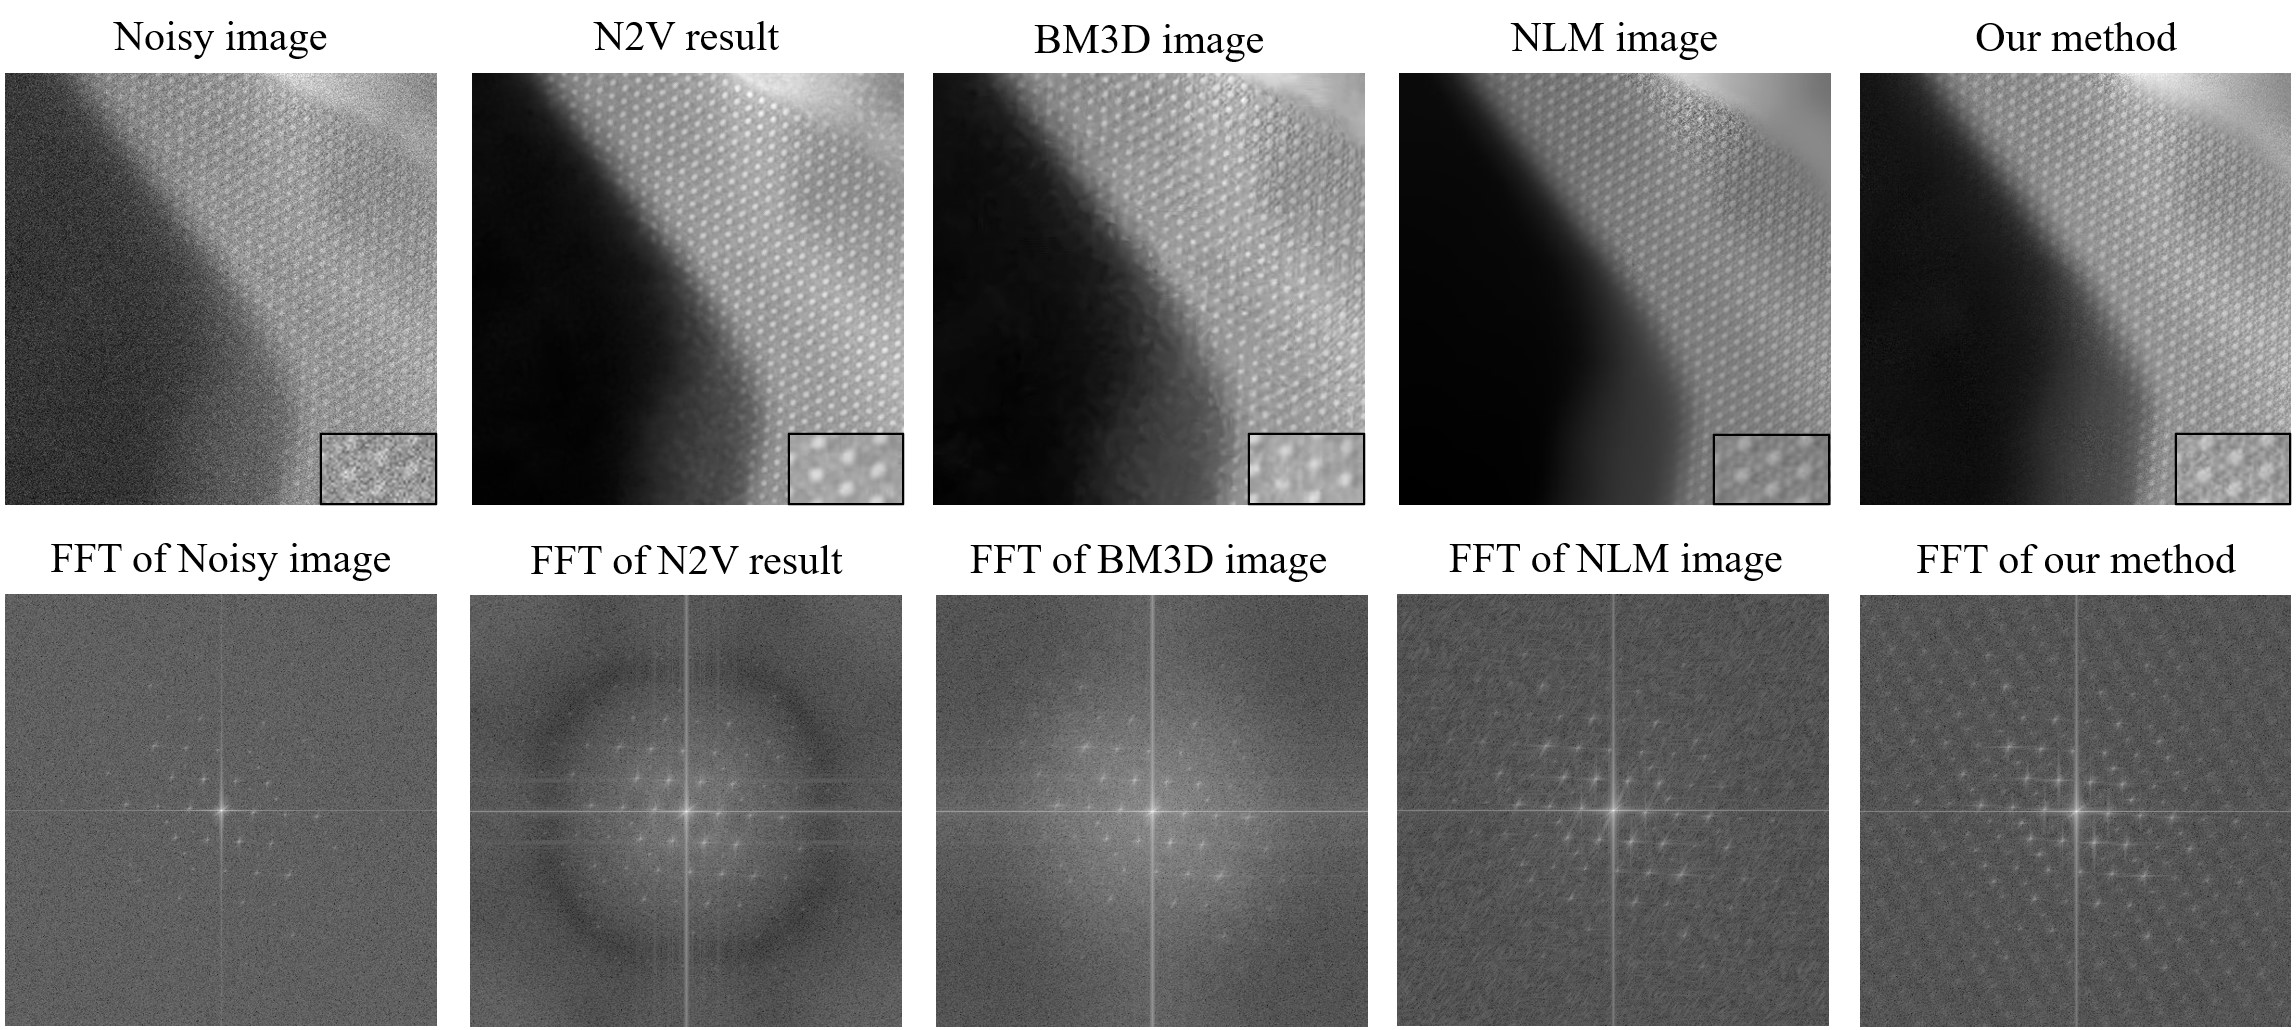
\includegraphics[scale=0.09]{./imgs/comparison.jpg}
	\caption{Comparison of results obtained from different methods}
	\label{fig:comparison}
\end{figure}


The proposed algorithm is mainly developed to denoise TEM images having repeated structures. The noisy image, the results from all the methods and their Fast Fourier transforms (FFT)\footnote{\url{https://numpy.org/doc/stable/reference/generated/numpy.fft.fft2.html}} can be seen in figure \ref{fig:comparison}. The FFT converts data from the spatial domain into the frequency domain. The white structures in the FFT represent information in the images. The signal corresponding to the low frequency components are represented at the center of the FFT and higher frequency components are present as we move away from the center. Noise corresponds to the high frequency components of the FFT and is present close to the edges.

The following can be concluded from the figure \ref{fig:comparison}:
\begin{itemize}
	\item The noisy image (of size 512*512 pixels) contains a lot of grainy structures which makes it hard to interpret the information. This is also reflected in the FFT, where the white structures are faintly visible at the center.
	
	\item N2V\cite{krull2019noise2void} is a self supervised, deep learning based image denoising method. N2V was trained with the patches of the noisy image. The training was done with $64*64$ patches, 100 epochs and a neighboring radius of 5. 
	
	The results from N2V show a decently reconstructed circular structures and the noise in the black region of the image has been removed fairly well. However, the substructures have not been reconstructed well which can be seen in the zoomed in sections. The FFT shows the enhanced white structures at the center and the edges mostly look dark representing the suppression of noise. 
	
	\item BM3D \cite{DBLP:journals/tip/BM3D} is one of the widely used classical denoising methods. BM3D uses collaborative filtering in the transform domain for denoising images and it is a non blind denoising method, which means that the standard deviation of the noise is required for denoising. The standard deviation was estimated with trial and error. The best results we obtained for a standard deviation of 0.06 for the normalized image.
	
	The results from BM3D are similar to that obtained from N2V. The denoising effect is visible but the images are still not very useful for further analysis. This is also supported by the Fourier transform.
	
	\item Non Local Means (NLM) \cite{bcm_nlm} is a conventional image denoising method that finds similar patches of images within a region and averages them to suppress noise. An NLM implementation\footnote{\url{https://scikit-image.org/docs/stable/auto_examples/filters/plot_nonlocal_means.html}} with a patch size of $46*46$, a search area of $100*100$ and a cut off distance of 0.36 was used. 
	
	The result shows a good level of denoising. The circular structures and sub structures between them are visible fairly well. At most regions, the the level of noise suppression is good. But at some regions, the existence of noise can still be seen. The FFT also shows stronger white structures supporting the indicating the enhancement of image features. Overall, the results look good and more interpretable. 
	
	\item Results with proposed denoising algorithm were obtained with a patch size of 46*46, a group size was between 5 and 100, and the clustering parameter, $c$ equal to 2.7 were used. 
	
	From the denoised result, it could be observed that the quality of denoising is marginally better than that from NLM. The image noise levels are suppressed fairly well and the information from the image can be well interpreted. The substructures between the circular structures are also better visible. From the FFT too, it can be seen that the white structures are more prominently visible. Some features can also be seen in the high frequency region which was previously not visible so well.
\end{itemize}

Apart from the qualitative improvement in the results, the proposed algorithm has a bigger advantage with regards to the computational time. The runtime of the proposed method for the images in figure \ref{fig:comparison} was 19.4 seconds, where as NLM, which was the closest to our results had a runtime of 171.4 seconds. This optimization in the runtime is particularly helpful when denoising image stacks from Transmission Electron Microscopy. The images in the stacks are \textbf{sometimes/often?} similar. In such cases, our algorithm not only matches the templates in the current image, but also the patches from other images in the stack. This significantly improves the quality of the results and with GPU computations, the computation speed is quite fast. For reference, the denoising of an image stack with 10 images of size 1024*1024 pixels took 281.8 seconds. The computations were carried out on a computer with 128 GB of RAM, Intel Xenon processor (16 CPUs), and Nvidia RTX6000 GPU.

\subsection*{Comparison with example images}


\subsection*{Confidence map}
From the above discussions, it can be observed that the algorithm can introduce artifacts. It is important to recognize this to determine if the denoised image is satisfactory. Since it is challenging to detect minute artifacts from Fourier analysis, a confidence map was developed. This confidence map is based on the variance within each cluster obtained after applying clustering. The variance should be small if the centroid is a good representation of its members. Also, a good centroid should not have any patterns in its variance. Patterns in the variance show that the centroid does not generalize its members well. 

The confidence map of the denoised image is calculated by combining the variances\cite{chan1982updating} for different centroids as they are back plotted. The overall variance map, i.e., the confidence map of a denoised image is as shown in figure \ref{fig:confidence_map}. This result has been produced for demonstration purpose with a very few initial \textit{reference patches} selected very close to each other. The bright regions in the confidence map correspond to the denoised image artifacts. For instance, a bright region can be seen in the confidence map at the top-right position. An artifact can be found by inspecting the same region on the denoised image. Similarly, irregularities in the black region on the left side of the denoised image can be recognized by the brighter regions of the confidence map.

\section*{Discussion}

The Discussion should be succinct and must not contain subheadings.
 

\bibliography{sample}

\noindent LaTeX formats citations and references automatically using the bibliography records in your .bib file, which you can edit via the project menu. Use the cite command for an inline citation, e.g.  \cite{Hao:gidmaps:2014}.

For data citations of datasets uploaded to e.g. \emph{figshare}, please use the \verb|howpublished| option in the bib entry to specify the platform and the link, as in the \verb|Hao:gidmaps:2014| example in the sample bibliography file.

\section*{Acknowledgements (not compulsory)}

Acknowledgements should be brief, and should not include thanks to anonymous referees and editors, or effusive comments. Grant or contribution numbers may be acknowledged.

\section*{Author contributions statement}

Must include all authors, identified by initials, for example:
A.A. conceived the experiment(s),  A.A. and B.A. conducted the experiment(s), C.A. and D.A. analysed the results.  All authors reviewed the manuscript. 

\section*{Additional information}

\subsection*{Algorithm}
\label{algorithms}

\begin{algorithm}
	\caption{Denoising Algorithm}
	\label{algorithm:denoising_algorithm}
	\begin{algorithmic}[1]
		\State \textbf{Input}: Noisy image
		\State \textbf{Result}: Denoised image
		\State \textit{imgs} $\gets$ loadImgs() ;
		\State set [\textit{templateSize, minGroupSize, maxGroupSize, clustParam}] ;
		\State \textit{refPatches} $\gets$ generate\_initial\_ref\_patches(\textit{imgs}, \textit{templateSize}) ;
		\State \textit{c} $\gets$ 15 ;
		
		\For{\textit{c} $\geq$ 0 \textbf{or} (check if the number of \textit{refPatches} in the last two iterations has changed)}
		
		\State \textit{tmpMatchResult} $\gets$ [ ]	;		
		
		\For{\textit{img} in \textit{imgs}}
		\For{\textit{refPatch} in \textit{refPatches}}
		
		\State \textit{tmpMatchResult}.append(template\_matching(\textit{img}, \textit{refPatch})) ;
		
		\EndFor
		\EndFor
		
		\State \textit{maxValue} $\gets$ max(\textit{tmpMatchResult}, axis=2) ;
		\State \textit{refPatchIndex} $\gets$ `\textit{refPatches}' index at \textit{maxValue} ;
		\State [\textit{sorted\_maxValue, positionX, positionY}] $\gets$ sortWithIdx(\textit{maxValue}); 
		\State \textit{t} = \textit{templateSize} ;
		\State \textit{list[\textit{idx},\textit{posX},\textit{posY}]} = [ ];
%%		\algstore{part1}
	%%\end{algorithmic}
%%\end{algorithm}
%%\begin{algorithm}
%%	\begin{algorithmic}[1]
%%		\algrestore{part1}
		
		\For{each \textit{s,posX,posY} in \textit{sorted\_maxValue, positionX, positionY}}
		\If{\textit{maxValue[posX,posY]} \textbf{not equal} 0}
		\State \textit{maxValue}[\textit{posX: posX}+($t/4$); \textit{posY: posY}+($t/4$)] $\gets$ 0 ;
		\State \textit{idx} $\gets$ \textit{refPatchIndex}[\textit{posX},\textit{posY}] ;
		\State \textit{list}.append([\textit{idx},\textit{posX},\textit{posY}]) ;
		\EndIf
		\EndFor
		
		\State [\textit{count,refPatchID}] $\gets$ count\_patches\_with\_same\_id(\textit{list});
		% \State \textit{max\_ind} = max(\textit{refPatchIndex}) ;
		
		\For{\textit{cnt,ID} in \textit{count,refPatchID}}
		\If{\textit{cnt} $\le$ \textit{minGroupSize}}
		\State \textit{list} $\gets$ delete(\textit{list}, \textit{ID});
		
		\ElsIf{\textit{cnt} $\ge$ \textit{maxGroupSize}}
		
		\State \textit{list} $\gets$ splitGroup(\textit{list}, \textit{ID}, \textit{maxGroupSize});
		
		%\For{\textit{l} in \textit{list}}
		%	\If{list[idx] == ind}
		%		\If{loopCounter == \textit{params}[\textit{maxGroupSize}]}
		%			\State \textit{loopCounter} = \textit{loopCounter} + 1
		%			\State \textit{list}[\textit{idx}] $\gets$ \textit{max\_ind}
		%			\State \textit{max\_ind} $\gets$\textit{ max\_ind} + 1
		%		\EndIf
		%	\EndIf
		%\EndFor
		
		\EndIf
		
		\EndFor
		
		\State \textit{refPatches} $\gets$ average\_patches\_with\_same\_id(\textit{list}) ;
		
		\State \textit{c} $\gets$ \textit{c}-1 ;
		\EndFor
		\State \textit{subGroup}[\textit{centroid, posX, posY}] = [ ];
		\For{\textit{refPatchID} in \textit{refPatches}}
		\State \textit{patches\_with\_sameRef} $\gets$ get\_patches\_with\_same\_id(\textit{list},\textit{refPatchID});
		\State \textit{numClusters} $\gets$ count(\textit{patches\_with\_sameRef})/\textit{clustParam} ;
		\State \textit{subGroup}.append(cluster(\textit{patches\_with\_sameRef, numClusters})) ;
		\EndFor
		\State \textit{gaussianWeight} $\gets$ createGaussianWeight();
		\State \textit{denoisedImg} $\gets$ backPlot(\textit{subGroup}, \textit{gaussianWeight});
	\end{algorithmic}
\end{algorithm}

\clearpage

%\begin{algorithm}
%	\caption{Algorithm for calculating variance}
%	\label{algorithm:variance_algorithm}
%	\begin{algorithmic}[1]
%		\State \textit{weight} $\gets$ \textit{weightA} + \textit{weightB} ;
%		\State \textit{delta} $\gets$ \textit{avgB} - \textit{avgA} ;
%		\State \textit{M2} $\gets$ (\textit{M2\_A} + \textit{M2\_B} + $delta^2$ *  \textit{weightA} * \textit{weightB}) / n ;
%		\State \textit{Var\_AB} = \textit{M2} / (\textit{n} - 1);
%	\end{algorithmic}	
%\end{algorithm}

\end{document}